\documentclass{beamer}
\let\vec\mathbf
\mode<presentation>
\usepackage{amsmath}
\usepackage{amssymb}
%\usepackage{advdate}
\usepackage{adjustbox}
%\usepackage{subcaption}
\usepackage{enumitem}
\usepackage{multicol}
\usepackage{mathtools}
\usepackage{listings}
\usepackage{url}
\usetheme{Boadilla}
\usecolortheme{lily}
\setbeamertemplate{footline}
{
  \leavevmode%
  \hbox{%
  \begin{beamercolorbox}[wd=\paperwidth,ht=2.25ex,dp=1ex,right]{author in head/foot}%
    \insertframenumber{} / \inserttotalframenumber\hspace*{2ex} 
  \end{beamercolorbox}}%
  \vskip0pt%
}
\setbeamertemplate{navigation symbols}{}
\providecommand{\nCr}[2]{\,^{#1}C_{#2}} % nCr
\providecommand{\nPr}[2]{\,^{#1}P_{#2}} % nPr
\providecommand{\mbf}{\mathbf}
\providecommand{\pr}[1]{\ensuremath{\Pr\left(#1\right)}}
\providecommand{\qfunc}[1]{\ensuremath{Q\left(#1\right)}}
\providecommand{\sbrak}[1]{\ensuremath{{}\left[#1\right]}}
\providecommand{\lsbrak}[1]{\ensuremath{{}\left[#1\right.}}
\providecommand{\rsbrak}[1]{\ensuremath{{}\left.#1\right]}}
\providecommand{\brak}[1]{\ensuremath{\left(#1\right)}}
\providecommand{\lbrak}[1]{\ensuremath{\left(#1\right.}}
\providecommand{\rbrak}[1]{\ensuremath{\left.#1\right)}}
\providecommand{\cbrak}[1]{\ensuremath{\left\{#1\right\}}}
\providecommand{\lcbrak}[1]{\ensuremath{\left\{#1\right.}}
\providecommand{\rcbrak}[1]{\ensuremath{\left.#1\right\}}}
\theoremstyle{remark}
\newtheorem{rem}{Remark}
\newcommand{\sgn}{\mathop{\mathrm{sgn}}}

\providecommand{\res}[1]{\Res\displaylimits_{#1}} 
\providecommand{\norm}[1]{\left\lVert#1\right\rVert}
\providecommand{\mtx}[1]{\mathbf{#1}}

\providecommand{\fourier}{\overset{\mathcal{F}}{ \rightleftharpoons}}
%\providecommand{\hilbert}{\overset{\mathcal{H}}{ \rightleftharpoons}}
\providecommand{\system}{\overset{\mathcal{H}}{ \longleftrightarrow}}
	%\newcommand{\solution}[2]{\textbf{Solution:}{#1}}
%\newcommand{\solution}{\noindent \textbf{Solution: }}align
\providecommand{\dec}[2]{\ensuremath{\overset{#1}{\underset{#2}{\gtrless}}}}
\newcommand{\myvec}[1]{\ensuremath{\begin{pmatrix}#1\end{pmatrix}}}

\title{Matrices in Geometry - 1.9.26}
\author{EE25BTECH11037  Divyansh}
\date{Aug, 2025}

\begin{document}

\maketitle


\section{Problem}
\begin{frame}
\frametitle{Problem Statement}
Find the value of P, if the point $\vec{A}\brak{0,2}$ is equidistant from point $\vec{B}\brak{3,P}$ and $\vec{c}\brak{p,5}$
\end{frame}

\section{Solution}
\begin{frame}{Solution}
   \textbf{Given: } 
$\vec{A}\myvec{0\\2}$, $\vec{B}\myvec{3\\P}$ and a point $\vec{C} \myvec{P\\ 5}$ such that $\vec{P}$ is equidistant from $\vec{A}$ and $\vec{B}$. 
\begin{align}
    \therefore \norm{\vec{A}-\vec{B}}=\norm{\vec{A}-\vec{C}}\\
    \text{On squaring both the sides, we get }\\
    \norm{\vec{A}-\vec{B}}^2=\norm{\vec{A}-\vec{C}}^2\\
    \myvec{\vec{A}-\vec{B}}^{\top}\myvec{\vec{A}-\vec{B}}=\myvec{\vec{A}-\vec{C}}^{\top}\myvec{\vec{A}-\vec{C}}\\
\end{align}
\end{frame}

\begin{frame}{Solution}
\begin{align}
\vec{A}^{\top}\vec{A} - 2\vec{A}^{\top}\vec{B} + \vec{B}^{\top}\vec{B} =\vec{A}^{\top}\vec{A} - 2\vec{A}^{\top}\vec{C} + \vec{C}^{\top}\vec{C}\\
    \norm{\vec{B}}^2 - \norm{\vec{C}}^2=2\vec{A}^{\top}\myvec{\vec{B}-\vec{C}}\\
    \norm{\myvec{3\\P}} - \norm{\myvec{P\\5}}=2\myvec{0 & 2}\myvec{3-P \\ P-5}\\
    9 + p^2 - p^2 -25 = 2\brak{0+2p-10}\\
    -16=4p - 20 \implies 4p =4 \implies p=1
\end{align}
\end{frame}



\section{Final Answer}
\begin{frame}{Final Answer}
\begin{align}
    \text{Hence, the final answer is }\fbox{p = 1} 
\end{align}
\begin{figure}
    \centering
    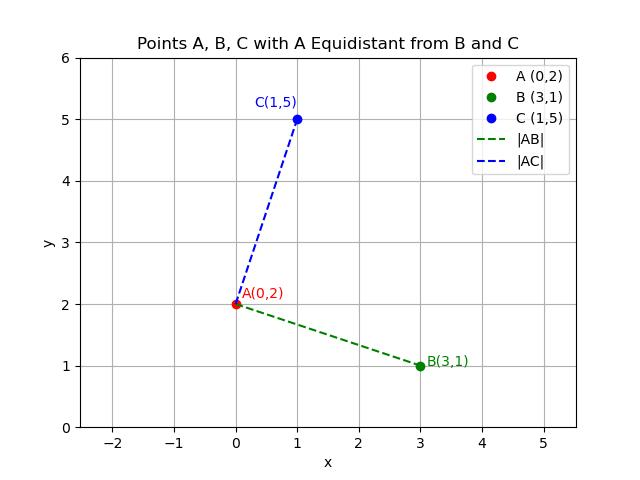
\includegraphics[width=0.6\columnwidth]{figs/1.jpg}
\end{figure}
\end{frame}
\end{document}